\documentclass{article}

\usepackage[margin=2.5cm]{geometry}

\usepackage[utf8]{inputenc}


\usepackage{graphicx}
\usepackage{fancyhdr}
\usepackage{fancyvrb}

\usepackage{tcolorbox}

\usepackage{listings}
\usepackage{xcolor}

\definecolor{codegreen}{rgb}{.2,0.6,0}
\definecolor{codegray}{rgb}{0.5,0.5,0.5}
\definecolor{codepurple}{rgb}{0.58,0,0.82}
\definecolor{codeblue}{rgb}{0,0.4,0.82}
\definecolor{codeorange}{rgb}{0.94,0.34,0.0}
\definecolor{backcolour}{rgb}{0.95,0.95,0.92}
\definecolor{backcolourgray}{rgb}{0.92,0.92,0.92}
\definecolor{codewhite}{rgb}{1,1,1}

\lstdefinestyle{mystyle}{
    backgroundcolor=\color{backcolourgray},   
    commentstyle=\color{codegreen},
    keywordstyle=\color{codeblue},
    numberstyle=\tiny\color{black},
    stringstyle=\color{codeorange},
    basicstyle=\ttfamily\footnotesize,
    breakatwhitespace=false,         
    breaklines=true,                 
    captionpos=b,                    
    keepspaces=true,                 
    %numbers=left,                    
    numbersep=5pt,                  
    showspaces=false,                
    showstringspaces=false,
    showtabs=false,                  
    tabsize=2,
    extendedchars=true,
    frame=single
    %, basicstyle=\footnotesize
}
\lstset{style=mystyle}

\usepackage{hyperref}
\hypersetup{
    colorlinks=true,
    linkcolor=blue,
    filecolor=magenta,      
    urlcolor=cyan,
}

\pagestyle{fancy}
\fancyhf{}
\rhead{Arquitectura de ordenadores. Practice 3.}
\lhead{Pablo Cuesta Sierra, Álvaro Zamanillo Sáez}
\cfoot{\thepage}



%\setlength{\parskip}{0.15cm}



\begin{document}


\title{Arquitectura de ordenadores. Practice 3.}
\author{Pablo Cuesta Sierra, Álvaro Zamanillo Sáez}
%\date{}
\maketitle

\begin{tcolorbox}
\tableofcontents
\end{tcolorbox}

\addcontentsline{toc}{subsection}{Exercise 0}
\subsection*{Exercise 0}

\lstinputlisting[]{files/0_3}

\addcontentsline{toc}{subsection}{Exercise 1}
\subsection*{Exercise 1}


\begin{figure}[h]
    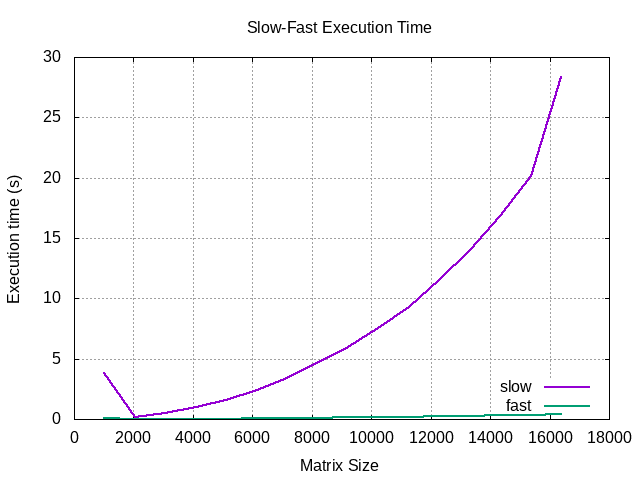
\includegraphics[scale=0.4]{../material_P3/slow_fast_time.png}
    \centering
    \caption{Search 8.}
    \label{slow_fast_time_means}
\end{figure}

\end{document}


\begin{lstlisting}[language=C, texcl=true]
    typedef struct Mine_struct_{
        long int target;
        long int begin; //índice por el que empieza a buscar el hilo
        long int end; //índice hasta el que el hilo busca (no incluido)
    } Mine_struct;  \end{lstlisting}